% -------------------------------------------------------------
% Source da minha Dissertação de Mestrado em Ciência Política (2/2015)
% -------------------------------------------------------------

% DOCUMENTO
\documentclass[12pt,oneside,a4paper,spanish,english,brazilian, sumario=abnt-6027-2012, chapter=TITLE ]{abntex2}

% CONFIGURACOES DO PPGPOL/UFRGS
\usepackage{PPGPOL}

% INFORMACOES
\titulo{Coalizões Governamentais Sobredimensionadas na América Latina, 1979-2012}
\author{Fernando Meireles}
\data{2015}
\instituicao{Universidade Federal do Rio Grande do Sul}
\departamento{Instituto de Filosofia e Ciência Humanas}
\programa{Programa de Pós-Graduação em Ciência Política}
\local{Porto Alegre}
\tipotrabalho{Dissertação (Mestrado)}
\orientador{Dr. Paulo Sérgio Peres}
\preambulo{Dissertação apresentada ao Programa de Pós-Graduação em Ciência Política do Instituto de Filosofia e Ciências Humanas da Universidade Federal do Rio Grande do Sul como requisito parcial para a obtenção do título de Mestre em Ciência Política.}

% TEXTO
\begin{document}
\pretextual
\imprimircapa
\imprimirfolhaderosto

% FICHA CATALOGRAFICA
\begin{fichacatalografica}
\vspace*{15cm} % Posição vertical
\centering CIP - Catalogação na Publicação
\vspace*{0.2cm}
\sffamily
\hrule % Linha horizontal
\begin{center} % Minipage Centralizado
\begin{minipage}[c]{12.5cm} % Largura
Meireles, Fernando\\
\hspace*{0.5cm} \imprimirtitulo / \imprimirautor. -- \imprimirlocal, \imprimirdata. \newline
\hspace*{0.5cm} \pageref{LastPage} f.\newline

\hspace*{0.5cm} \imprimirorientadorRotulo ~Paulo Sério Peres\\

\hspace*{0.5cm} \imprimirtipotrabalho ~-- \imprimirinstituicao, \imprimirdepartamento, \imprimirprograma, Porto Alegre, BR-RS, \imprimirdata.\\

\hspace*{0.5cm} 1. Coalizões governamentais. 2. Presidencialismo. 3. Relações Executivo-Legislativo. I. Peres, Paulo Sério, orient. II. Título.
\end{minipage}
\end{center}
\hrule
\end{fichacatalografica}
\clearpage

% FOLHA DE APROVACAO
%\begin{folhadeaprovacao}

  \begin{center}
    {\large\scshape\imprimirautor}

    \vspace*{\fill}\vspace*{\fill}
    {\bfseries\large\MakeUppercase {\imprimirtitulo}}
    \vspace*{\fill}
    
    \hspace{.45\textwidth}
    \begin{minipage}{.5\textwidth}
    \SingleSpacing\small
        \imprimirpreambulo
    \end{minipage}%
    \vspace*{\fill}
   \end{center}
    
   \centering Trabalho aprovado em XX de fevereiro de 2015.

   \assinatura{Prof. Dr. Paulo Sérgio Peres \\ (Orientador)} 
   \assinatura{Professor1}
   \assinatura{Professor2}
   \assinatura{Professor3}
      
   \begin{center}
    \vspace*{0.5cm}
    {\large\scshape\imprimirlocal}
    \par
    {\large\scshape\imprimirdata}
    \vspace*{1cm}
  \end{center}
  
\end{folhadeaprovacao}
\clearpage

% AGRADECIMENTOS
%\begin{agradecimentos}
Agradecimentos vão aqui.

\end{agradecimentos}

% RESUMO
\begin{resumo}
Nos últimos anos, a maior parte da literatura sobre as relações executivo-legislativo em sistemas presidencialistas vem enfatizando o papel da formação de coalizões governamentais, através da distribuição de ministérios, na obtenção de maiorias legislativas. Contudo, essas coalizões formadas raramente são iguais, já que umas são maiores e, por causa disso, mais propensas à problemas coordenativos e de agência. Mas o que explica a decisão de um presidente de incluir mais ou menos partidos em seu gabinete? Com um banco de dados original contendo informações sobre 168 coalizões na América Latina entre 1979 e 2012, este artigo testa algumas das hipóteses correntes sobre o fenômeno. Entre outros, os resultados mostram que legislativos fortes e efetivos, presidentes que dispõem de maiores poderes legislativos e maior fragmentação partidária aumentam a probabilidade de ocorrência de coalizões sobredimensionadas em diversas especificações.

\vspace{\onelineskip}
\noindent
\textbf{Palavras-chaves}: Coalizões governamentais;  Presidencialismo; Relações Executivo-Legislativo.
\end{resumo}
\newpage

% ABSTRACT
\begin{resumo}[Abstract]
 \begin{otherlanguage*}{english}
Research on executive-legislative relations in presidential systems have emphasized how presidents use cabinet appointments to form and manage government coalitions in the absence of majority legislative support. Yet not all coalitions look alike, as some are bigger and, consequently, more prone to agency and coordination problems than others. But what shapes presidents' decision to include more or less parties in their coalitions? While several hypotheses exist in the literature, few have been tested in a systematic fashion, none focusing on why surplus coalitions form. This paper intends to fill this gap by examining an original time-series cross-sectional dataset comprising 168 unique coalitions in all 18 Latin American presidential countries since 1979. In particular, I find that strong and effective assemblies, presidents with great legislative powers and high levels of party fragmentation are associated with oversized coalitions in different model specifications.

\vspace{\onelineskip}
\noindent
\textbf{Key-words}: Government coalitions;  Presidentialism; Executive-Legislative relations.
 \end{otherlanguage*}
\end{resumo}
\newpage

% LISTAS
\pdfbookmark[0]{\listfigurename}{lof}
\listoffigures*
\clearpage
\pdfbookmark[0]{\listtablename}{lot}
\listoftables*
\clearpage

% SIGLAS
%\begin{siglas}
  \item[MWC] Minimum Winning Coalition
  \item[NEPP] Número Efetivo de Partidos Parlamentares

\end{siglas}
\clearpage

% SUMARIO
\pdfbookmark[0]{\contentsname}{toc}
\tableofcontents*
\clearpage

\textual
\pagestyle{simple}

% INTRODUCAO
\section{Introdução}
\label{sec:introduction}

Que presidentes frequentemente recorrem à formação de coalizões para governar não constitui mais novidade alguma. Nos últimos anos, o que a literatura sobre o presidencialismo vem procurando explicar é, justamente, como isso ocorre. A tese básica que emergiu a partir de então é a de que essas coalizões são administradas através de um conjunto de ferramentas, uma \textit{toolbox}, que pode ser estrategicamente empregada pelo presidente para incentivar a cooperação e coordenar a ação dos partidos no Congresso (CHAISTY et. al., \citeyear{chaisty2014}). Dentre outros, poder de agenda (uso de decretos legislativos e pedidos de urgência, etc.), controle sobre a execução e formulação do orçamento (\textit{pork}) e distribuição de ministérios (\textit{coalition goods}) seriam os principais instrumentos que permitiriam a superação dos "perigos"{} inerentes aos regimes com separação de poderes. Como o uso dessas ferramentas varia entre países e contextos, entretanto, é algo que levanta uma série de questões.

No caso específico da distribuição de ministérios, por exemplo, os presidentes devem decidir qual será o tamanho da coalizão e quão bem recompensados serão os seus parceiros. Por sua vez, essa decisão é, ela própria, parcialmente determinada por outros fatores. Sobre isto, a literatura não vai muito além de destacar que a existência de decretos legislativos e vetos parciais podem incentivar um presidente a governar de forma imperial, distribuindo poucos ministérios (AMORIM NETO,  \citeyear{neto2000}, \citeyear{neto2006}; COX e MORGENSTERN, \citeyear{cox2001}); e que o número mínimo de partidos que o presidente precisa incorporar também depende da posição que ele ocupa no espectro ideológico e do número de cadeiras que seu partido dispõe (CHEIBUB, \citeyear{cheibub2007}; FIGUEIREDO et al., \citeyear{figueiredo2012}; NEGRETTO, \citeyear{negretto2006}). Contudo, isso não explica como essas variáveis interagem com outras ferramentas da \textit{toolbox}\footnote{Ao analisar o \textit{trade-off} entre incentivos seletivos e distribuição de ministérios no gerenciamento das coalizões dos governos FHC e Lula, Raile, Pereira e Power (\citeyear{raile2010}) constituem exceção, embora não abordem o principal problema desenvolvido no restante deste artigo.}, tampouco nos fornecem uma explicação completa para a variação no tamanho das coalizões governamentais em sistemas presidencialistas.

Isso é ainda mais sintomático quando se procura entender o surgimento de coalizões sobredimensionadas, nas quais existem mais partidos do que o necessário para se obter maioria absoluta no congresso. Em primeiro lugar, porque, como Riker (\citeyear{riker1962}) demonstrou, mais membros numa coalizão significa menos cargos à disposição de cada membro do governo. À luz disso, formar coalizões sobredimensionadas seria um erro. Segundo, porque em coalizões fragmentadas e heterogêneas as políticas ideais de cada partido dificilmente podem ser realizadas simultaneamente, o que com frequência gera custos de transação e conflitos entre estes (AXELROD, \citeyear{axelrod1970}). E, terceiro, porque delegar ministérios com jurisdições específicas pode incentivar cada ministro a buscar políticas que sirvam apenas ao seu partido, mesmo que isso prejudique os demais parceiros da coalizão (SAALFELD, \citeyear{saalfeld2000}; MARTIN e VANBERG, \citeyear{martin2011}; FREITAS, \citeyear{freitas2012})\footnote{Uma leva de estudos argumenta que estes problemas de \textit{moral hazard} decorrentes dessa relação agente-principal são contornáveis (e. g., AMORIM e TAFNER, \citeyear{neto2002}; FREITAS, \citeyear{freitas2012}; STR\O{}M et al., \citeyear{strom2010}). Mesmo assim, essas correções trazem custos: esse é ponto principal do argumento aqui utilizado.}. Considerando a frequência com que ocorrem - Figueiredo et al. (\citeyear{figueiredo2012}, p. 847) reportam que mais de 35\% dos governos na América Latina entre 1979 e 2011 foram supermajoritários -, portanto, cabe perguntar: por que presidentes propõem, e partidos aceitam integrar, coalizões sobredimensionadas? Por que aqueles não cedem apenas um número suficiente de ministérios para obter maioria? E, em todo o caso, os mesmos fatores que explicam o surgimento de coalizões menores também explicam as maiores? E qual é a relação entre coalizões grandes e demais ferramentas da \textit{toolbox}? Apesar da importâncias dessas questões, as respostas na literatura a essas perguntas são vagas e estudos comparados, inexistentes.
 
Neste artigo, procuro exatamente preencher esta lacuna. Com um banco de dados que cobre todos os 18 países presidencialistas da América Latina após a terceira onda da democratização, testo algumas daquelas respostas presentes na literatura com análise multivariada. Ao invés da mais recorrente, a de que, antecipando a indisciplina dos partidos que o sustentam, os presidentes aumentariam o tamanho de suas coalizões, sugiro uma outra, relacionada às necessidades de gerenciamento da coalizão: a de que quanto mais forte for o poder legislativo, mais partidos na coalizão serão necessários para formar um cartel legislativo. Um exemplo disso ocorre no governo Dilma I, enquanto escrevo esta introdução. 

Insatisfeitos com o governo e com a política de alianças regionais do PT, alguns parlamentares lançaram ofensivas que, no plenário e na Comissão de Agricultura, Pecuária, Abastecimento e Desenvolvimento Rural da Câmara, respectivamente, derrubou um decreto da Presidente e convocou dois Ministros\footnote{O ESTADO DE SÃO PAULO. "Câmara derruba decreto de conselho popular de Dilma". Disponível em: \url{http://goo.gl/rJPuXB}. Acesso em: 3 de novembro de 2014.} \footnote{CONGRESSO EM FOCO. "Oposição supera bloqueio na Câmara e convoca dois ministros". Disponível em:~\url{http://goo.gl/W7ZNEY}. Acesso em: 3 de novembro de 2014}. Formalmente, essas ações foram possíveis porque ao Presidente da Câmara cabe estabelecer a agenda de votações, e a uma maioria simples dos membros de cada Comissões aprovar pedidos para depoimentos. Atualmente, esses espaços são controlados pela base governista. Sendo assim, qualquer ação contra o governo, nestes espaços, só ocorrem se contarem com o suporte de membros da coalizão\footnote{Sobre isto, a nota do Congresso em Foco é ilustrativa: "\textit{Da base aliada, poucos deputados se manifestaram contra a convocação dos ministros}. Márcio Macedo (PT-SE) sugeriu que os pedidos fossem transformados em convite.[...] Porém, como a maioria da comissão faz parte da bancada ruralista, atualmente em pé de guerra com o Planalto, as tentativas dos governistas em modificar os requerimentos acabou fracassada." (Ênfase minha).}. Em qualquer outro caso, a oposição não prevalece.

Independentemente do desfecho, ambos os exemplos ilustram perfeitamente como o sistema de comissões e a organização do legislativo podem oferecer amplas prerrogativas de veto e revisão legislativa, controle da agenda e mesmo investigação de outros poderes. Quanto mais numerosos e efetivos forem esses espaços, mais parlamentares serão necessários para os controlar. Em outras palavras, coalizões governamentais, quando funcionam, também servem para obter a cooperação de legislativos fortes o suficiente para contrariar os interesses de um presidente.

No restante do artigo, procedo da seguinte forma. Após discutir brevemente os principais parâmetros nos modelos sobre formação de coalizões governamentais no parlamentarismo, discuto algumas adaptações destes para o presidencialismo e os problemas que geraram na seção~\hyperref[sec:revisao]{2}. Na seção~\hyperref[sec:FAZER]{3}, introduzo as hipóteses a serem testadas sobre os determinantes das coalizões sobredimensionadas na Amérila Latina. Na seção~\hyperref[sec:FAZER]{4}, discuto o método e apresento os dados utilizados, que cobrem o período entre 1978 a 2010 e incluem todos os 18 países presidencialistas da América Latina -- incluso os da América Central, frequentemente ignorados pela literatura comparada. Nas seções~\hyperref[sec:FAZER]{5} e~\hyperref[sec:FAZER]{6}, apresento e discuto os resultados. Por fim, seguem as conclusões.

\newpage

% SEGUNDA SECAO
\chapter{O tamanho das coalizões}
\label{chap:revisao}

Governos de coalizão são comuns no parlamentarismo. Segundo a explicação corrente, a razão disso estaria nos incentivos gerados pela dependência do executivo em relação ao legislativo. Quando o partido do primeiro-ministro não dispõe de maioria, o apoio de uma coalizão, mesmo que tácito, é necessário para evitar que o governo caia (LAVER e SHEPSLE, \citeyear{laver1996}; STR\O{}M, \citeyear{strom1990}). Desse modo, por não estar em questão as causas dessas coalizões, os estudos sobre o parlamentarismo puderam se voltar principalmente ao problema da variação entre elas: quantos partidos participam, quais deles e por quanto tempo (Cf., LAVER e SCHOFIELD \citeyear{laver1998}). Nos primeiros estudos sobre o tema no presidencialismo, ao contrário, a possibilidade mesma de surgirem governos de coalizão é que estava em causa (CHEIBUB, \citeyear{cheibub2002}; FOWERAKER, \citeyear{foweraker1998}; LINZ, \citeyear{linz1990}; MAINWARING, \citeyear{mainwaring1993}; STEPAN e SKACH, \citeyear{stepan1993}). No que segue, procuro argumentar que, justamente por isso, outros aspectos das coalizões governamentais no presidencialismo foram muito menos explorados. O tamanho delas é um exemplo.

\section{Tamanho das coalizões no parlamentarismo}

O que um partido ganha entrando numa coalizão? E quais fatores explicam por que algumas coalizões possuem mais partidos do que outras? A literatura sobre o parlamentarismo, mais antiga e extensa, nos fornece um bom ponto de partida para encontrar algumas dessas respostas. Grosso modo, três são as principais variáveis explicativas apontadas por ela: \textit{distribuição de cadeiras}, \textit{preferências ideológicas} e \textit{instituições}. As instituições porque estruturariam o processo de negociação e montagem de governos e, assim, delimitariam o número de coalizões que poderiam ser efetivamente formadas (STR\O{}M et al., \citeyear{strom1994}); já o número de cadeiras e a posição ideológica dos partidos, porque indicariam quais dessas coalizões seriam mais viáveis (AXELROD, \citeyear{axelrod1970}).

O marco inicial dessa literatura é bastante conhecido. Políticos procurariam usufruir de cargos públicos, que são bens escassos e de uso exclusivo, e, para tanto, formariam uma maioria na assembléia para controlar o governo. Dentre todas as coalizões que os permitiriam fazer isso, a ótima seria aquela que contaria com o mínimo de membros, a \textit{minimum winning coaltion} (MWC) (RIKER, (\citeyear{riker1962}). Na perspectiva dos políticos, isso seria vantajoso porque minimizaria o número de pessoas com quem eles teriam que dividir cargos, que são fixos no curto-prazo. Como todos enfrentam a mesma situação, a cooperação prospera e coalizões mínimas, mas capazes de satisfazer o critério de decisão majoritária, surgiriam. Embora não tenha sido o primeiro a formular esse modelo\footnote{Antes dele, Gamsom (\citeyear{gamson1961}) o formalizou de forma ampla; ele próprio, contudo, afirma que seu modelos inspira-se numa tradição alguns anos mais antiga, oriunda das primeiras contribuições à teoria dos jogos.}, Riker (\citeyear{riker1962}) o aplicou à situação concreta de formação de maiorias numa assembleia e derivou daí uma proposição bastante precisa sobre a coalizão que surgiria dada um distribuição de cadeiras\footnote{Cabe notar, do que fica implícito nesta proposição, que basta apenas a defecção de um membro da coalizão para que esta perca o controle do \textit{spoil}. Na prática, contudo, uma coalizão alternativa deve substituir a anterior para que este \textit{spoil} mude de mãos. Isto ocorre porque, na maioria dos países parlamentaristas, no caso de ausência de uma maioria alternativa, um governo \textit{caretaker} assume, geralmente composto por membros do governo anterior e comprometida em não alterar o \textit{status quo} (LAVER e SCHEPSLE, \citeyear{laver1996}, p. 47-8)}.

A simplicidade desse modelo \textit{office-seeking} \footnote{Para uma discussão sobre outros modelos \textit{office-based}, ver Martin e Stevenson (\citeyear{martin2001}) e Crombez (\citeyear{crombez1996}).}, entretanto, foi justamente o principal objeto de crítica da literatura subsequente. Entre outros, Luebbert (\citeyear{luebbert1986}) e Str\o{}m (\citeyear{strom1990}) mostraram que coalizões minoritárias não apenas surgiam com frequência, mas também que estas eram tão estáveis e poderiam durar por tanto tempo quanto suas correlatas majoritárias. Deste modo, Riker criou um \textit{puzzle} enorme: por que a oposição permite a sobrevivência de gabinetes minoritários? Ou bem existiria alguma compensação (\textit{side-payment}) aos partidos de fora do governo, ou então a utilidade destes seria derivada de outros locais.
 
Na esteira desse problema, emergiu a ideia de que não apenas cargos importavam, mas também a ideologia. A não ocupação de cargos poderia ser compensada, ou mesmo substituída, pela implementação de uma agenda legislativa da preferência dos partidos. Uma primeira explicação para isso seria a de que os membros de uma coalizão, por exemplo, buscariam diminuir os conflitos entre eles. Como nem sempre numa barganha dois partidos conseguem firmar acordo - seja por desconfiança mútua, falta de informações sobre as consequências do acordo, entre outros -, dois partidos quaisquer em coalizão poderiam incluir nela todos aqueles que estivessem situados entre eles numa escala ideológica unidimensional para amenizar esse problema, o que poderia gerar coalizões maiores do que as \textit{MWC} (AXELROD, 1970)\footnote{A explicação de Axelrod (1970) é a seguinte: se o potencial de conflito entre dois partidos aumenta quanto maior for a distância entre eles numa dimensão qualquer, e se o potencial de conflito numa coalizão é a média dos potenciais de conflitos entre todos os pares não repetidos de partidos, coalizões com menor variação nas preferências dos seus membros, isto é, coalizões mais homogêneas, gerariam maiores ganhos de estabilidade.}. Com isso, a manutenção da coalizão se tornaria mais fácil porque o novo integrante assumiria, de forma prática, o papel de mediano da coalizão, evitando que este tivesse que ser negociado. No caso das coalizões mínimas, a explicação poderia ser ainda mais direta: um partido de oposição pode simplesmente se beneficiar das políticas do governo e, por isso, não ter incentivos para derrubá-lo. Entre outros, a principal vantagem de fazer isso seria a de se poupar de desgastes com a administração pública, particularmente quando medidas impopulares precisam ser implementadas. Antecipando esse comportamento, o partido encarregado de formar uma coalizão, o \textit{formateur}, pode estrategicamente manter partidos ideologicamente próximos fora do governo e reter inteiramente o executivo. Tacitamente, contudo, uma coalizão existiria (STR\O{}M, \citeyear{strom1990}).

Distribuição de cadeiras e de preferências, portanto, podem influenciar o tamanho de uma coalizão, mas não fazem isso num vácuo institucional. Um conjunto de regras estrutura o processo de formação de gabinetes no parlamentarismo, determinando as estratégias de cada partido. Enquanto que, em tese, uma assembléia fragmentada oferece diversas possibilidades de coalizão, certas regras podem alterar drasticamente esse número (STR\O{}M et al., \citeyear{strom1994}). Por exemplo, dependendo de como o partido \textit{formateur} é escolhido, outros partidos podem recusar propostas de integrar a coalizão -- desde que tenham chances de se tornar o próximo \textit{formateur} caso as negociações em curso falhem, o que justamente lhes dá incentivos para não cooperar (AUSTEN-SMITH e BANKS, \citeyear{austen1988}). A divisão do governo em jurisdições específicas comandadas por ministérios, por sua vez, também pode dificultar a acomodação de muitos partidos num gabinete, pois torna difícil o monitoramento de cada ministério individualmente e aumenta as chances de que surjam conflitos intragovernamentais (LAVER e SHEPSLE, \citeyear{laver1996}). Deste modo, a consideração das regras que delimitam os cursos de ação disponíveis aos partidos seriam necessárias para tornar mais precisos os modelos sobre formação de gabinetes multipartidários.

Em suma, de acordo com essa literatura discutida, o contexto institucional e o número e as preferências dos partidos explicariam boa parte da variação no tamanho das coalizões formadas no parlamentarismo. O número de cadeiras seria um bom indicador da necessidade do partido \textit{formateur} buscar ou não uma coalizão e do número de partidos em coalizão necessários para se obter maioria. Preferências ideológicas, por outro lado, apontariam para como os partidos governariam e, portanto, seriam bons indicadores da probabilidade de que dois partidos quaisquer viessem a cooperar. Dependendo da posição e do número de cadeiras dos demais, coalizões mínimas ou sobredimensionadas podem surgir. Por fim, as regras que estruturam o processo de formação de coalizões e exercício do governo também deveriam ser levadas em conta para lidar com variações entre países e contextos, bem como para entender como a sequência de movimentos e as opções disponíveis a cada partido levam a equilíbrios diferentes dos que modelos \textit{office} ou \textit{policy-seeking} isoladamente indicariam. 


\section{Tamanho das coalizões no presidencialismo}

Ao contrário da literatura sobre o parlamentarismo, os estudos sobre sistemas presidencialistas até pouco tempo afirmavam que coalizões governamentais não deveriam surgir. Dois argumentos principais sustentariam essa conclusão. O primeiro é o de que, legitimados pela maioria dos eleitores, presidentes não dependeriam do apoio do legislativo para manter seus cargos. Essa seria a essência da dinâmica \textit{winner-takes-all} inerente ao presidencialismo (LINZ, \citeyear{linz1990}; LINZ e VALENZUELA, \citeyear{linz1994}; RIGGS, \citeyear{riggs1988}). O segundo argumento, desenvolvido por outra geração de comparativistas, é o de que certos aspectos institucionais comuns ao presidencialismo latino-americano dificultariam o surgimento de coalizões (MAINWARING, \citeyear{mainwaring1993}; SHUGART e CAREY, \citeyear{shugart1992}; STEPAN e SKACH, \citeyear{stepan1993}). Representação proporcional para eleições legislativas tornaria bastante provável que o partido do presidente não contasse com apoio legislativo de uma maioria. Sistemas eleitorais inclusivos, por outro lado, gerariam incentivos para a personalização e a regionalização das campanhas eleitorais, o que em último caso enfraqueceria a coesão dos partidos políticos e dificultaria a formação e a manutenção de coalizões. Deste modo, os presidentes da região não teriam incentivos para cooperar com as assembleias, preferindo antes contorná-las ou usar incentivos seletivos para formar coalizões legislativas \textit{ad hoc} (COX e MORGENSTERN, \citeyear{cox2001}; JONES, \citeyear{jones1995})\footnote{Reconstituir este debate está fora do escopo deste artigo. Boas revisões, entretanto, podem ser encontradas em Cheibub (\citeyear{cheibub2007}), Power (\citeyear{power2010}) e Negretto (\citeyear{negretto2006}).}.

Como essa premissa de ausência de cooperação entre executivo e legislativo colocava em causa a própria estabilidade democrática e a governabilidade dos países da América Latina, os primeiros estudos sobre o presidencialismo buscaram invariavelmente explorar as condições favoráveis à formação de governos multipartidários ao invés das diferenças entre estes. Passados alguns anos do início deste debate, hoje sabemos que coalizões governamentais são comuns e que auxiliam na aprovação da agenda presidencial, na diminuição de conflitos intergovernamentais e na sustentação de presidentes que enfrentam crises econômicas ou protestos populares (ÁLVAREZ e MARSTEINTREDET, \citeyear{alvarez2010}; CHEIBUB, \citeyear{cheibub2007}; CHEIBUB et al., \citeyear{cheibub2004}; HOCHSTETLER, \citeyear{hochstetler2006}; NEGRETTO, \citeyear{negretto2006}; PÉREZ-LIÑÁN, \citeyear{perez2007})\footnote{Na Colômbia e na Venezuela, assembleias constituintes foram convocadas e, durante seus trabalhos, dissolveram o congresso. Ainda que não tenha sido por intervenção militar, como o fracassado auto-golpe de Fujimori, no Peru, estas dissoluções não eram diretamente previstas pelas respectivas constituições –- ao contrário da uruguaia, que prevê tal prerrogativa, apesar de que, na prática, ela não seja usada (SHUGART e CAREY, \citeyear{shugart1992}, p. 127)}. Recentemente, também surgiram estudos mostrando que coalizões de diferentes tamanhos trazem consequências distintas, como promover a autonomia de agências regulatórias quando são estabelecidas, aumentar o grau de obstrução legislativa à agenda do presidente e facilitar a implementação de reformas estruturais (ALTMAN e CASTIGLIONI, \citeyear{altman2008}; HIROI e RENNÓ, \citeyear{hiroi2014}; MELO e PEREIRA, \citeyear{melo2013}). Mas, apesar desses avanços, à exceção de uns poucos estudos que analisam a composição e a estabilidade de gabinetes presidencialistas comparativamente (e. g., AMORIM NETO, \citeyear{neto2006}; FIGUEIREDO et al., \citeyear{figueiredo2012}; MARTINEZ-GALLARDO, \citeyear{martinez2012}), ainda sabemos pouco sobre o que explica essas diferenças no tamanho das coalizões que são formadas no Continente em primeiro lugar.

Em parte, o tamanho das coalizões poderia ser considerado função exclusiva da decisão dos presidentes, já que eles possuem a prerrogativa de nomear os ministros no presidencialismo. Contudo, esse dificilmente é o caso. A montagem de um gabinete multipartidário envolve a interação estratégica de diversos atores com preferências, poder de barganha e prerrogativas institucionais diferentes. Em decorrência disso, segundo Cheibub (\citeyear{cheibub2007}), a formação de uma coalizão é um jogo no qual os presidentes fazem propostas para os potenciais parceiros considerando os custos e a utilidade de tê-los cooperando e a probabilidade de eles aceitarem essas propostas. Se todos os jogadores procurarem implementar políticas públicas e obter cargos, coalizões surgiriam exceto quando as preferências ideológicas do presidente fossem tão extremas que nenhum partido obtivesse vantagem ao integrar o gabinete; ou quando o presidente estivesse centralmente localizado no espectro ideológico e fosse naturalmente o ponto de convergência da maioria. Em outras palavras, ainda que sejam eleitos separadamente e muitas vezes contem com amplos poderes legislativos, presidentes não escolhem arbitrariamente suas coalizões, já que as preferências dos demais partidos e o contexto no qual as negociações ocorrem produzem incentivos que determinam parcialmente os resultados do processo.

Da evidência disponível sobre governos de coalizão no presidencialismo, a maioria é consistente em mostrar que certos fatores de fato influenciam o tamanho das coalizões. Utilizando observações anuais dos gabinetes de 14 países da América Latina onde o partido dos incumbentes dispunha de menos de 50\% dos votos, Figueiredo et al. (\citeyear{figueiredo2012}) testaram algumas das hipóteses sobre a ocorrência de coalizões minoritárias, aquelas que não possuem maioria de apoio no congresso. Entre outros, eles mostram evidências de que vetos parciais e vetos difíceis de serem derrubado aumentam a probabilidade de surgirem coalizões minoritárias; por outro lado, assembleias fragmentadas e o efeito do ciclo eleitoral diminuiriam estas probabilidades. Já com análises \textit{time-series}, tanto Raile et al. (\citeyear{raile2010}) quanto Acosta e Polga-Hecimobich (\citeyear{acosta2011}) mostram que no Brasil e no Equador, respectivamente, o uso estratégico das emendas parlamentares pode compensar a cooperação dos membros da coalizão e evitar perdas de suporte legislativo ou mesmo a deserção de algum partido. Entretanto, outros estudos sugerem que, ao invés de cooperarem, presidentes podem usar de seus poderes legislativos para simplesmente contornar as assembleias: por exemplo, presidentes que contam com a prerrogativa de expedir decretos legislativos tendem a distribuir menos proporcionalmente ministérios entre seus parceiros de coalizão e a ter gabinetes menores e mais instáveis (AMORIM NETO, \citeyear{neto2006}; FIGUEIREDO et al., \citeyear{figueiredo2012}; MARTINEZ-GALLARDO, \citeyear{martinez2012}) \footnote{Qualificando esse efeito dos decretos legislativos, Negretto (\citeyear{negretto2004}) afirma que, onde existem, os presidentes só poderiam usá-los efetivamente quando controlam o membro pivotal do congresso, isto é, quando contam com uma base suficiente para impedir a aprovação de vetos - como foi o caso dos Presidentes Alfonsín e Menem na Argentina. Na ausência desta condição, expedir decretos funcionaria apenas como uma ferramenta de coordenação e delegação, reduzindo e transferindo os custos da tomada de decisões do congresso para o executivo}.
 
Enfim, apesar de estes estudos certamente ampliarem o nosso entendimento de como governos de coalizão funcionam, ainda não sabemos quais fatores explicam as variações entre eles. Coalizões podem ter diversos tamanhos e composições ideológicas diferentes, dependendo da decisão do presidente. Contudo, esta decisão, conforme argumentado, é parte de um jogo que envolve mais atores e um contexto que restringe o conjunto de estratégias disponíveis a cada um. Sobre isto, a teorização e as evidências sobre governos multipartidários na América Latina tendem a supervalorizar as experiências de alguns poucos países do Cone Sul, grosso modo, e não nos fornecem proposições específicas sobre a formação coalizões sobredimensionadas -- o que contrasta com a literatura sobre o parlamentarismo, onde o estudo deste tipo de coalizão já recebeu várias contribuições (Cf., VOLDEN e CARRUBA, \citeyear{volden2004}). Se governos de coalizão são podem surgir no presidencialismo e no parlamentarismo por razões semelhantes (Cf.CHEIBUB et al., \citeyear{cheibub2004}; CHEIBUB, \citeyear{cheibub2007}), falta ainda, portanto, testar se fatores comuns aos dois sistemas também são capazes de explicar a variação no tamanho das coalizões: o que, especificamente, um presidente ganha ao incluir mais partidos em seu gabinete, apesar dos custos de ter de dividir mais cargos e de barganhar com mais partidos? Qual é a influência que a relação entre executivo e legislativo desempenha na ocorrência desse fenômeno? E por que em alguns países estes tipos de coalizão não são formadas, como nos da América Central, e em outros, como Brasil e Chile, são formadas com frequência? No restante do artigo, procuro justamente contribuir para este debate através da análise dos determinantes da ocorrência de coalizões sobredimensionadas no presidencialismo latino-americano.


\newpage

% TERCEIRA SECAO
\chapter{Desenho de Pesquisa}
\label{chap:analise}

\documentclass{letter}
\usepackage{tikz}
\usetikzlibrary{patterns}
\usepackage{caption}
\usepackage{subcaption}

\def\firstcircle{(2.4,3.2) circle [radius=1.9]}
\def\secondcircle{(3,4) circle [radius=1]}
\def\thirdcircle{(4,5) circle [radius=1]}
\def\ponto{(3,5) circle [radius=0.06]}

\tikzset{
        hatch distance/.store in=\hatchdistance,
        hatch distance=10pt,
        hatch thickness/.store in=\hatchthickness,
        hatch thickness=2pt
    }

    \makeatletter
    \pgfdeclarepatternformonly[\hatchdistance,\hatchthickness]{flexible hatch}
    {\pgfqpoint{0pt}{0pt}}
    {\pgfqpoint{\hatchdistance}{\hatchdistance}}
    {\pgfpoint{\hatchdistance-1pt}{\hatchdistance-1pt}}%
    {
        \pgfsetcolor{\tikz@pattern@color}
        \pgfsetlinewidth{\hatchthickness}
        \pgfpathmoveto{\pgfqpoint{0pt}{0pt}}
        \pgfpathlineto{\pgfqpoint{\hatchdistance}{\hatchdistance}}
        \pgfusepath{stroke}
    }
\begin{document}

\begin{tikzpicture}
\begin{scope}[fill opacity=0.5]
\clip \thirdcircle;
\fill[pattern=flexible hatch, hatch distance=5.5pt, hatch thickness=0.35pt] \secondcircle;
\end{scope}
\fill[black] \ponto node[above]{$SQ$};
\draw[thick] \firstcircle node[below]{A};
\draw[thick] \secondcircle node{P};
\draw[thick] \thirdcircle node{C};
\draw[very thick,<->] (0,6) -- (0,1) -- (7,1);
\end{tikzpicture}
\end{document}


\section{Dados e método}

Examino os determinantes das coalizões governamentais sobredimensionadas com um banco de dados contendo informações sobre 168 coalizões governamentais únicas\footnote{Coalizões únicas são todas aquelas em que a composição partidária de um gabinete se manteve constante -- o que evidentemente engloba como coalizão gabinetes unipartidários.} em todos os 18 países presidencialistas da América Latina\footnote{Estes países são: Argentina (1983-2012), Bolívia (1982-2012), Brasil (1985-2012), Chile (1990-2012), Colômbia (1978-2012), Costa Rica (1978-2012), El Salvador (1994-2012), Equador (1979-1995, 1997-2005), Guatemala (1996-2011), Honduras (1982-2008, 2010-2012), México (1988-2011), Nicarágua (1997-2006), Panamá (1991-2008), Paraguai (1993-1997, 1999-2011), Peru (1980-2008), Rep. Dominicana (1996-2009), Uruguai (1985-2012) e Venezuela (1979-2001). As fontes utilizas para compilar todas as variáveis utilizadas são descritas no Apêndice A.}. Os dados cobrem o período que vai de 1979 até 2012, totalizando 439 observações no formato país-ano. Além da vantagem óbvia do aumento na amostra e na variação nos preditores, a inclusão dos países da América Central -- frequentemente ignorados pela literatura sobre o tema -- também me permite testar hipóteses elaboradas para os países do Cone Sul num contexto mais amplo.

\subsection{Variável dependente: coalizões sobredimensionadas}

Antes de classificar as coalizões de acordo com seus tamanhos, é necessário definir governo de coalizão. Seguindo outros estudos (e. g., AMORIM NETO, \citeyear{neto2006}; FIGUEIREDO et al., \citeyear{figueiredo2012}; MARTINEZ-GALLARDO, \citeyear{martinez2012}), o critério aqui utilizado para identificá-los é a filiação partidária dos ministros das principais pastas de cada país. A principal vantagem deste é tornar possível a repetição da coleta de dados, já que não deixa margem a erros de imputação. Por outro lado, o procedimento possui um maior problema: o suporte legislativo dado ao governo por um partido que possui membros no gabinete não é automático. Ministros nem sempre são recrutados pelas conexões ou influência legislativa que possuem; em outros casos, não são reconhecidos pelos seus partidos como representantes legítimos. Sem levar isso em conta, falsos positivos, isto é, governos erroneamente classificados como de coalizão, acabariam sendo compilados. Para contornar este problema, consultei especialistas em alguns dos países incluídos na amostra e outras três bases de dados sobre governos de coalizão para checar cada observação\footnote{Os dados que serviram de base me foram gentilmente cedidos por Octavio Amorim Neto e Cecília Martinez-Gallardo. Após compilar os casos remanescentes a partir das fontes descritas no Apêndice A, chequei parte dos resultados com os dados de Cheibub (\citeyear{cheibub2007}), Chasquetti (\citeyear{chasquetti2001}) e Saez e Montero (\citeyear{alcantara2008}). De todo o modo, para alguns países, sobretudo dos Andes e da América Central, os resultados ou não coincidiram ou não eram precisos. Nestes casos, pedi para os seguintes especialistas confirmarem a composição dos gabinetes e indicar se eram ou não de coalizão: Ivana Grace Deheza (Bolívia); Felipe Botero (Colômbia); Evelyn Villareal Fernandez e Jorge Vargas Cullel (Costa Rica); Alvaro Artiga e Nivaria Ortega (El Salvador); Eduardo Dargent e Paula Munoz Chirinos (Peru); e Rosario Espinal (Rep. Dominicana).}. Sempre que os dados originais divergiram dos de outras bases e estudos, a classificação final dos especialistas foi adotada. Feito isto, o número de partidos e cadeiras de cada coalizão foram compilados a partir da composição partidária corrigida de cada gabinete.

A existência de coalizões sobredimensionadas foi mensurada de duas formas. Primeiro, através de uma variável dicotômica que assume o valor 1 sempre que ao menos um dos membros da coalizão pudesse ser removido sem perda de maioria no congresso ou, em países bicamerais, na câmara baixa. Esta é a operacionalização convencional de coalizões \textit{surplus} (e. g., CROMBEZ, \citeyear{crombez1996}; MARTINEZ-GALLARDO, \citeyear{martinez2012}; VOLDEN e CARRUBBA, \citeyear{volden2004}). Para captar maior variação e testar a robustez dos resultados, entretanto, uma segunda variável conta o número de partidos que poderiam ser removidos sem perda de \textit{status} majoritário\footnote{Obviamente, as maiorias requeridas para aprovação de leis ordinárias varia entre os países incluídos na amostra: em alguns, a maioria absoluta dos membros presentes é necessária; em outros, a maioria simples dos membros presentes (MONTERO, \citeyear{montero2013}). De qualquer forma, se em N votações o número de presentes for estipulado de maneira aleatória, quanto maior for esse N maior será o número de vitorias do partido/coalizão com maioria legislativa; e, em última instância, qualquer votação poderá ser vencida desde que o total de parlamentares do lado majoritário seja mobilizado.}.

\subsection{Variáveis independentes}

Como dito anteriormente, as três principais hipóteses discutidas destacam o arranjo institucional e o contexto que estruturam a relação executivo-legislativo como os principais fatores que a explicam a formação de coalizões sobredimensionadas. Especificamente, elas preveem que a existência destas coalizões varia de acordo com os poderes legislativos do presidente, a força do congresso e demais fatores que influenciam a quantidade e as preferências de cada partido.

Para avaliar o efeito dos poderes legislativos dos presidentes, utilizo o índice desenvolvido por Negretto (\citeyear{negretto2013}) feito a partir de um modelo de variável latente estandardizado com valores de 0 a 100. O índice resume 14 indicadores categóricos de poder presidencial, como poder de veto e possibilidade de iniciar referendos. Quanto maiores os valores neste índice, mais forte é o presidente e, portanto, menos incentivos ele teria para formar coalizões \textit{surplus}. De qualquer modo, pode-se alegar que nem todos os poderes presidenciais geram incentivos para a formação de coalizões. Por isso, também utilizo outras três alternativas para mensurar aspectos diretamente relevantes dos poderes presidenciais. A primeira é um indicador da disponibilidade da prerrogativa de veto presidencial, que assume o valor de 1 quando presidente pode vetar parcialmente um projeto, 0.5 quando pode vetar totalmente um projeto e 0 quando não dispõe de poder algum; a segunda é um indicador do poder presidencial de expedir decretos legislativos que assume um valor máximo de 1 quando o presidente que também varia de 0, na ausência desta prerrogativa, a 1. Ambas as variáveis foram tomadas de Negretto (\citeyear{negretto2013}). Adicionalmente, também uso uma \textit{dummy}, tomada de Cheibub (\citeyear{cheibub2007}), para mensurar o poder orçamentário do presidente que assume o valor de 1 quando este domina o processo, isto é, quando é capaz de iniciar propostas orçamentárias sem sofrer vetos do congresso ou quando a falha em aprovar uma proposta alternativa beneficia o presidente.

Quanto à força do congresso, isto é, à capacidade do legislativo de impedir mudanças no \textit{status quo} e de fiscalizar e checar o executivo, não existe solução clara. Estudos comparados sobre o legislativo na América Latina são poucos, bem como a disponibilidade de índices para mensurar e classificar suas capacidades (ALEMAN, \citeyear{aleman2013}). Para capturar este fator, assim, recorro ao \textit{polcon3}, uma índice que atribui valores entre 0, quando mudanças no \textit{status quo} não sofrem qualquer tipo de impedimento, e  1, quando o \textit{winset} do \textit{status quo} é vazio (HENISZ, \citeyear{henisz2002}). Ele é especialmente adequado porque leva em consideração o número de casas legislativas, a fragmentação e a coincidência na distribuição partidária em cada uma delas ao atribuir os \textit{scores}. O ponto negativo desta variável, contudo, é o de não considerar a capacidade de fiscalização do congresso, que também pode ser usada para induzir a cooperação do executivo. Para mensurar isto, incluo alternativamente uma variável sobre a efetividade do legislativo calculada a partir da resposta de altos executivos no setor privado à pergunta “Quão efetivo é o parlamento/congresso nacional na produção legiferante e fiscalização?”, feita pelo \textit{Global Competitiveness Report} do \textit{World Economic Forum} (STEIN et al., \citeyear{stein2006}). Os valores vão de 1, “muito ineficiente”, a 7, “muito eficiente”. Apesar de não estar livre de problemas, esta é a principal solução em estudos que consideram o poder do legislativo (e. g., ALEMAN e TSEBELIS, \citeyear{aleman2011}; MARTINEZ-GALLARDO, \citeyear{martinez2012}). 

As variáveis contextuais utilizadas são três. A primeira delas é o Número Efetivo de Partidos Parlamentares, que mensura a probabilidade de que dois parlamentares selecionados aleatoriamente pertençam ao mesmo partido elevada na menos um, i. e., $NEPP = (\sum_{i=1}^{n} C_{i}^2)^{-1}$ , onde $C_{i}$ é a percentagem de cadeiras do partido $i$\footnote{O NEPP foi preferido ao invés do índice de Fracionalização de Rae porque, ao contrário deste, não possui um teto no valor máximo.}. Num congresso mais fragmentado, é esperado que presidentes incluam mais partidos em seus gabinetes para explorar problemas coordenativos entre estes, conforme estipula a Hipótese 2. As outras duas variáveis captam o efeito da distribuição de preferências ideológicas, que afetam o ambiente de negociações e determina os custos de cooperação. Para gerá-las, cada partido com mais de 5\% de cadeiras no congresso de cada país em cada ano foi codificado numa escala que vai de 1 a 5, da esquerda à direita; na sequência, esses \textit{scores} foram ponderados pela percentagem de cadeiras dos partidos e a variável resultante foi centrada. As informações sobre as posições dos partidos foram extraídas de três fontes diferentes, dando origem a três versões de cada variável\footnote{As fontes são descritas no Apêndice A.}. \textit{Polarização no congresso} é simplesmente o desvio-padrão da distribuição dessas preferências em cada país-ano e mensura o grau de polarização no congresso. \textit{Extremismo do presidente}, por sua vez, é igual a posição do partido do presidente menos a média das posições de todos os partidos ao quadrado, i. e., $(p_{1}~ -~\bar{p})^2$, dividido pelo somatório do quadrado da posição de cada partido menos aquela mesma média, i. e., \textit{Extremismo} $= \frac{(p_{1}~ -~\bar{p})^2}{\sum_{i=2}^{n-1} (p_{i} ~ - ~ \bar{p})^2}$, onde $p_{i}$ é a posição ideológica do partido $i$ e $i = 1$ indica o partido do presidente. Este procedimento é necessário para tornar comparáveis os \textit{scores} entre países e anos, já que a distância do presidente em relação à média do congresso depende da posição de todos os partidos: mantendo a distância do presidente igual, maior polarização o aproxima relativamente do centro; ao contrário, menor polarização o torna relativamente mais distante (Cf. CROMBEZ, \citeyear{crombez1996}).
 
Também incluo alguns controles. \textit{Ciclo eleitoral} é igual ao tempo em anos restantes de mandato dividido pela duração total do mandato presidencial e serve para mensurar o efeito do ciclo eleitoral sobre o tamanho das coalizões. Com a proximidade das eleições, partidos teriam incentivos para sair da coalizão e disputá-las de forma independente (ALTMAN, \citeyear{altman2000}; SHUGART e CAREY, \citeyear{shugart1992}). De todo o modo, este resultado também depende da popularidade do presidente, já que a decisão de abandonar a coalizão baseia-se na utilidade de ir à oposição (MARTINEZ-GALLARDO, \citeyear{martinez2012}). Infelizmente, não existem dados sobre a aprovação presidencial em todos os países analisados. Como \textit{proxy}, entretanto, utilizo o logaritmo, atrasado em um ano, da taxa de inflação anual do \textit{World Development Indicators}\footnote{Disponível em: \url{http://data.worldbank.org/data-catalog/world-development-indicators}. Acesso em: 28/01/2015.}. A expectativa do seu efeito é simples: quanto maior a inflação, menos incentivos os partidos de oposição têm para ir ao lado governista. Por fim, também controle os resultados pela percentagem de cadeiras do partido do presidente.

\subsection{Modelos}

Para estimar a probabilidade de surgirem coalizões sobredimensionadas $Y_{i, t}$ num país $i$ num ano $t$, o modelo básico utilizado é

\begin{equation}
Pr(Y_{i, t} = 1 \mid X_{i, t}) = \Lambda(X_{i, t}\beta + s(t) + \varepsilon_{i, t})
\end{equation}
\noindent
onde $\Lambda(\cdot)$ é a função de distribuição cumulativa logística; $X$ é a matriz que contém as variáveis independentes; e $s(\cdot)$ é um polinômio cúbico usado para controlar a dependência temporal na variável dependente (Cf. CARTER e SIGNORINO, \citeyear{carter2010}). Como apenas 6 dos 18 países presidencialistas do Continente tiveram coalizões sobredimensionadas no período, incluir efeitos-fixos removeria arbitrariamente boa parte das observações. Ainda que ajudassem a captar heterogeneidades não-observadas, os custos de incluí-los, portanto, seriam grandes. 
 
A análise que segue também não está livre de problemas de endogeneidade comuns na política comparada. Para dar maiores garantias de que os resultados não se devem a problemas como este, portanto, realizo também uma série de \textit{robust checks} -- como o uso de uma amostra reduzida e efeitos fixos, de modelos binomiais negativos e da inclusão de diversos controles.





\newpage

% QUARTA SECAO
\chapter{Resultados}
\label{chap:resultados}

Os resultados dos principais modelos estimados estão na~\hyperref[table:tabela1]{Tabela 1}. Os modelos 1, 2 e 3 são versões do modelo básico: o primeiro utiliza o índice de poder presidencial composto por 14 indicadores; o 2 utilizada apenas três destes indicadores; e o 3 inclui uma variável de efetividade do legislativo. Os modelos 4 e o 5 são regressões binomiais negativas com o número de partidos adicionais como variável dependente

\begin{table}[htb]
\IBGEtab{\caption{Determinantes da ocorrência de coalizões governamentais sobredimensionadas na América Latina, 1979-2012}
\label{table:tabela1}
}{%
\begin{tabular}{lccccc}
\toprule
{} & \textbf{Modelo 1} & \textbf{Modelo 2} & \textbf{Modelo 3} & \textbf{Modelo 4} & \textbf{Modelo 5} \\
\midrule
Número efetivo de partidos & 0.21 & 0.29** & 0.36 & 0.30*** & 0.18** \\
{} & (0.14) & (0.14) & (0.32) & (0.11) & (0.08) \\
Força do legislativo (Polcon3) & 3.55** & 4.19** & 6.56** & 2.86** & 2.65** \\
{} & (1.83) & (2.16) & (3.42) & (1.16) & (1.62) \\
Poder presidencial & 0.04** & & & 0.03*** & \\
{} & (0.02) & & & (0.01)&  \\
Efetividade do legislativo & & & 1.01* & & 1.64*** \\
{} & & & (0.57) & & (0.43) \\
Poder de veto &  & -3.02 & 1.13 & & -4.7** \\
{} &  & (2.11) & (7.32) & & (2.43) \\
Controle do orçamento &  & 0.28 & 0.29 & & -1.82** \\
{} &  & (0.93) & (1.12) &  & (0.88) \\
Decreto legislativo &  & 1.92 & 3.32 & & -0.72 \\
{} & & (1.63) & (3.43) & & (0.98) \\
Extremismo do presidente & -1.15** & -1.3*** & -1.81** & -0.93*** & -0.55** \\
{} & (0.45) & (0.42) & (0.65) & (0.26) & (0.23) \\
Polarização no congresso & -9.06** & -6.63* & -17.06** & -4.93** & -10.63*** \\
{} & (3.82) & (3.52) & (7) & (2.35) & (2.98) \\
Ciclo eleitoral & 1.77** & 1.95** & 2.98** & 0.52* &  0.83*\\
{} & (0.92) & (0.98) & (1.5) & (0.31) & (0.48) \\
\% de cadeiras do presidente & 8.17*** & 9.14*** & 10.83*** & 3.93** & 2.42 \\
{} & (2.7) & (2.97) & (3.82) & (1.58) & (1.6) \\
Inflação_{log} & -0.42* & -0.76** & -1.27** & -0.01** & -0.21*** \\
{} & (0.22) & (0.33) & (0.65) & (0.09) & (0.08) \\
$t$ & -4.47*** & -4.2*** & -3.92*** & & \\
{} & (0.82) & (0.85) & (1.37) & & \\
$t^{2}$ & 0.71*** & 0.64*** & 0.60** & & \\
{} & (0.15) & (0.15) & (0.25)& & \\
$t^{3}$ & -0.03*** & -0.03*** & -0.03** & & \\
{} & (0.01) & (0.01) & (0.1) & & \\
Log-likelihood & -53.14 & -52.29 & -26.47 & -218.12 & -148.72 \\
Clusters & 102 & 102 & 82 & 102 & 82 \\
N & 421 & 421 & 328 & 421 & 328 \\
\bottomrule
\end{tabular}%
}{ %
\nota{$\ast\ast\ast p<0.01; \ast\ast p<0.05; \ast p< 0.1$. Os modelos foram estimados por \textit{maximum likelihood}. Erros-padrão robustos com \textit{cluster} para os presidentes entre parênteses. As constantes foram omitidas e a variável inflação foi atrasada.}
}
\end{table}

Conforme indica a tabela, todos os modelos são consistentes com as hipóteses 1 e 2, e apresentam os sinais esperados em quase todas as variáveis. Congressos capazes de bloquear mudanças no \textit{status quo} e mais fragmentados aumentam a probabilidade de vermos um gabinete sobredimensionado -- ainda que a estimativa do efeito desta  última varie bastante entre os modelos. Inflação elevada, proximidade das eleições e o tamanho da representação do partido do presidente no congresso também apresentam efeitos significantes e condizentes com as expectativas: quando os preços sobem, presidentes perdem popularidade (presume-se) e se tornam menos capazes de administrar coalizões grandes; já no início de seus mandatos, ou quando seus partidos possuem grandes bancadas, o contrário ocorre.

Presidentes mais extremados ideologicamente e congressos mais polarizados diminuem a probabilidade de surgirem grandes coalizões, o que intuitivamente faz sentido: coalizões com partidos próximos ideologicamente são mais fáceis de serem geridas; do mesmo modo, presidentes mais moderados têm menores dificuldades de atrair partidos aos seus gabinetes. A maior surpresa fica por conta da variável que mensura o poder presidencial, que é significativa nos modelos 1 e 4 mas apresenta efeito contrário do que previa a Hipótese 3, isto é, presidentes que contam mais poderes legislativos são \textit{mais} propensos a formar coalizões sobredimensionadas. Verificando o efeito de apenas alguns dos indicadores que de poder presidencial mencionados pela literatura como importantes, entretanto, o modelo 2 mostra que nenhum deles é significativo. Controle do processo orçamentário e poder de expedir decretos apresentam sinais esperados nos modelos 2 e 3, mas não os mantêm nas outras especificações. Por seu turno, o efeito do poder de veto é o mais inconsistente de todos, embora seja significativo e apresente o sinal esperado no modelo 5: de acordo com este, quando possui o poder de evitar mudanças no \textit{status quo} possivelmente contrárias aos seus interesses, presidentes são menos impelidos à formar gabinetes grandes.

Das variáveis de interesse, as com efeito mais substantivo são poder presidencial, polarização no congresso, força do legislativo e, nos três primeiros modelos, tempo transcorrido desde o último gabinete sobredimensionado. Centrando todas as variáveis do modelo 1 e estipulando o número de anos desde o último gabinete sobredimensionado, \textit{t}, em dois anos\footnote{Como existe grande dependência temporal na variável dependente, qualquer valor inferior ou superior a dois tende a determinar a probabilidade prevista. Portanto, dois é o número de anos que mais ou menos aproxima 50\% de probabilidade do \textit{outcome} de interesse.}, a diferença na probabilidade prevista de um presidente com o máximo de poderes legislativos na amostra (95) formar uma coalizão sobredimensionada e outro com mínimo de poderes (22.45) é de 9\%; por sua vez, o congresso mais forte da amostra gera uma probabilidade de surgir uma coalizão \textit{surplus} de 6\% a mais do que o congresso mais fraco; e, por fim, o menor valor de polarização ideológica registrada está associada a uma probabilidade de 16\% a mais do que o mais polarizado\footnote{Todas estas são estimativas médias, e algumas delas não atingem níveis convencionais de significância. Usando os valores da amostra, e não a média das variáveis, essas mesmas probabilidades são de, respectivamente, 8\%, 9\% e 20\%.}. A~\hyperref[fig:figura1]{Figura 1} ajuda a ilustrar este último efeito. Especificamente, ela mostra que a probabilidade de surgir uma coalizão sobredimensionada diminui conforme a polarização no congresso aumenta.

\begin{figure}[htb]
	\label{fig:figura1}
	\caption{Efeito da polarização no congresso sobre a probabilidade de ocorrência de coalizões sobredimensionadas (IC 95\%)}
	\begin{center}
	    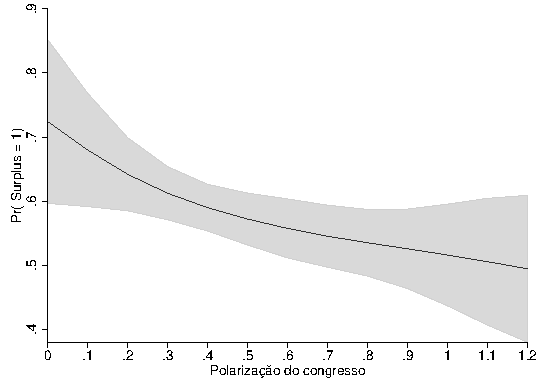
\includegraphics[scale=1.5]{polarization.pdf}
	\end{center}
	\legend{Fonte: elaboração própria.}
\end{figure}


Outra variável de interesse com efeito mais substantivo é o Número Efetivo de Partidos Parlamentares. Como previa a Hipótese 2, congressos com mais partidos aumentam a oferta de parceiros potenciais e permitem aos presidentes explorar problemas coordenativos entre estes. De acordo com o modelo 2, a estimativa deste efeito é considerável e corrobora aquela hipótese: com as demais variáveis na média e $t = 2$, um congresso com NEPP igual a 2 possui 4\% de probabilidade de ter uma coalizão sobredimensionada; já com NEPP igual a 10, a probabilidade aumenta para 34\%. De qualquer modo, como a incerteza nessa estimativa é muito elevada, outra abordagem melhor ilustra esse efeito. Simulando os coeficientes e a matriz de variância-covariância do modelo 2 mil vezes \footnote{Utilizei o conjunto de macros CLARIFY, de Tomz et al., (\citeyear{tomz2003}), para gerar essas quantidades de interesse.}, a distribuição das probabilidades de surgirem coalizões sobredimensionadas quando o NEPP é de 2 e de 10, respectivamente, é apresentada na~\hyperref[fig:figura2]{Figura 2}. Como é possível verificar, a diferença entre a média das estimativas oculta os platôs mais salientes nas extremidades, mais condizentes com a hipótese inicial.

\begin{figure}[htb]
	\label{fig:figura2}
	\caption{Distribuição do efeito do Número Efetivo de Partidos Parlamentares sobre a probabilidade de ocorrência de coalizões sobredimensionadas}
	\begin{center}
	    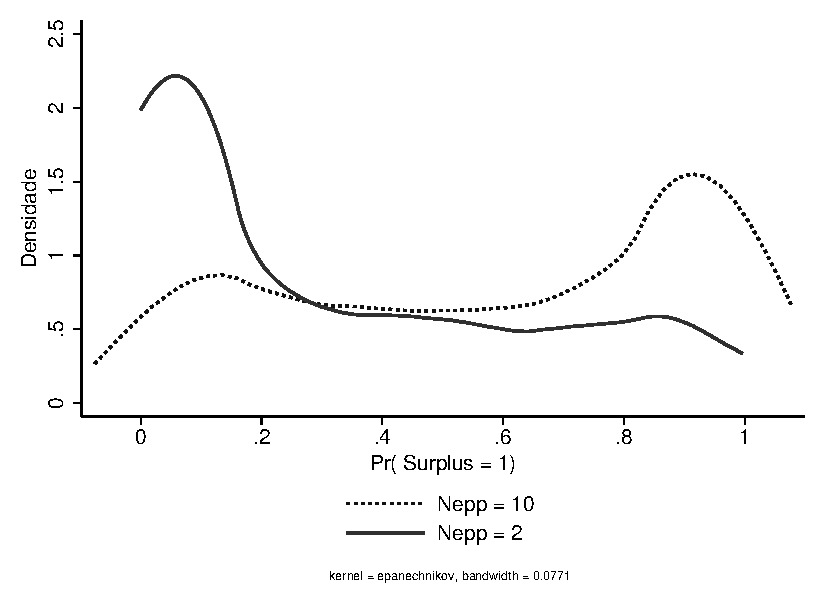
\includegraphics[scale=1.1]{enp.pdf}
	\end{center}
	\legend{Fonte: elaboração própria.}
\end{figure}


Por fim, o efeito da dependência temporal de um ano para outro nos três primeiros modelos merecem um comentário. Quando o gabinete imediatamente anterior é sobredimensionado, a probabilidade de que o corrente também seja é de 65\%, de acordo com o modelo 1. Como seria de se esperar, gabinetes multipartidários frequentemente duram mais do que um ano, mas esse efeito de continuidade desaparece rapidamente: quando a distância temporal entre um gabinete sobredimensionado e outro é maior do que dois anos, a probabilidade deste também ser sobredimensionado é quase 0. Embora não desapareçam repentinamente, portanto, governos com coalizões grandes parecem não durar mais do que um mandato de 4 anos, em média.

Com apenas um indicador binário para captar a presença de coalizões sobredimensionadas, gabinetes com apenas um pequeno partido adicional, como muitos dos formados pela \textit{Concertación}, no Chile, são indistinguíveis de outros com mais partidos. Para contornar isso, os modelos 4 e 5, que empregam o número de partidos excedentes na coalizão como variável dependente. Os principais resultados estão de acordo com os modelos anteriores. O poder presidencial atinge significância, mas, novamente, no sinal oposto ao que previa a Hipótese 3. Fixando as demais variáveis do modelo 4 na média, um presidente com o \textit{score} máximo no índice de poder presidencial aumenta em 0.34 o número esperado de partidos adicionais na coalizão; já utilizando os valores originais da amostra, fixando apenas o valor da variável de interesse, mesmo número chega a quase 1. A~\hyperref[fig:figura3]{Figura 3} exibe este efeito para todos os valores do índice de poder presidencial.

\begin{figure}[htb]
	\label{fig:figura3}
	\caption{Efeito do poder presidencial sobre o número esperado de partidos adicionais na coalizão}
	\begin{center}
	    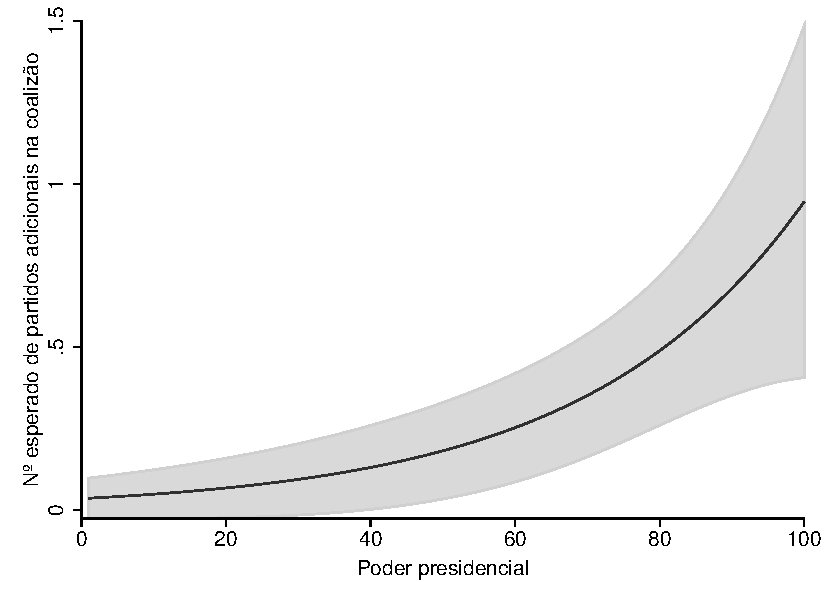
\includegraphics[scale=1]{negretto.pdf}
	\end{center}
	\legend{Fonte: elaboração própria.}
\end{figure}


No modelo 5, Número Efetivo de Partidos Parlamentares mantém o efeito positivo, agora sobre o valor esperado de partidos adicionais na coalizão, e adquire uma estimativa mais precisa. De todo o modo, de acordo com o modelo 5, a mudança de 2 para 10 partidos efetivos gera um aumento esperado de 0.08 partidos adicionais na coalizão, com as demais variáveis fixadas na média. Quanto à efetividade do legislativo, apesar da redução na amostra por ela não estar disponível para todos os casos, a diferença entre o congresso mais efetivo e o menos efetivo é de 0.33 partidos adicionais. Isoladamente, a variável com efeito mais substantivo no modelo 5 continua sendo a polarização no congresso: a maior polarização registrada na amostra provoca um aumento de 0.51 partidos adicionais esperados maior do que o menos polarizados, todo o resto fixo.

Nos modelos 6, 7, 8 e 9 da~\hyperref[table:tabela2]{Tabela 2}, apenas os seis países com ocorrência de coalizões sobredimensionadas no período foram analisados, gerando, assim, uma amostra mais balanceada\footnote{Em nenhum deles a variável \textit{Efetividade do Legislativo}, já que, por ter observações incompletas, a sua inclusão reduziria ainda mais o tamanho da amostra.}. Embora os resultados não se alterem substancialmente, o descarte das demais observações implica que esta amostra não é minimamente representativa da América Latina e, por isso, os resultados não podem ser generalizados. 

\begin{table}[htp]
\IBGEtab{\caption{Determinantes da ocorrência de coalizões governamentais sobredimensionadas em seis países da América Latina, 1979-2012}
\label{table:tabela2}
}{%
\begin{tabular}{lcccc}
\toprule
{} & \textbf{Modelo 6} & \textbf{Modelo 7} & \textbf{Modelo 8} & \textbf{Modelo 9} \\
\midrule
Número efetivo de partidos & 0.38* & 0.20 & 0.35*** & 0.29*** \\
{} & (0.21) & (0.23) & (0.09) & (0.07) \\
Força do legislativo (Polcon3) & 5.98*** & 6.5*** & 1.65* & 1.7** \\
{} & (1.83) & (1.75) & (0.88) & (0.79) \\
Poder presidencial (Negretto) & 0.05** & & 0.02** &  \\
{} & (0.02) & & (0.01) &  \\
Poder de veto & & -7.69 & & -2.29 \\
{} & & (4.97) &  & (1.68) \\
Controle do orçamento & & 1.84 &  & 0.58 \\
{} & & (1.24) &  & (0.72) \\
Decreto legislativo & & -0.41 &  & -0.11 \\
{} & & (2.12) &  & (0.64) \\
\% de cadeiras do presidente & 9.88*** & 9.69*** & 3.66**  & 3.54*** \\
{} & (3.12) & (2.82) & (1.58) & (1.34) \\
Extremismo do presidente & -1.74*** & -1.59*** & -0.65** & -0.72*** \\
{} & (0.54) & (0.43) & (0.27)  & (0.16) \\
Polarização no congresso & -3.42 & 0.37 & -0.22 & 1.07 \\
{} & (4.14) & (5.12) & (2.46) & (2.28) \\
Ciclo eleitoral & 1.08** & 1.19** & 0.47 & 0.54* \\
{} & (0.55) & (0.55) & (0.37) & (0.31) \\
Inflação_{log} & -0.48** & -0.64* & -0.26** & -0.31*** \\
{} & (0.23) & (0.34) & (0.1) & (0.09) \\
Log-likelihood & -67.7 & -66.15 & -159.46 & -158.18 \\
Clusters & 36 & 36 & 36 & 36 \\
N & 154 & 154 & 154 & 154 \\
\bottomrule
\end{tabular}%
}{%
\nota{$\ast\ast\ast p<0.01; \ast\ast p<0.05; \ast p< 0.1$. Os modelos foram estimados por \textit{maximum likelihood}. Erros-padrão robustos com \textit{cluster} para os presidentes entre parênteses. As constantes foram omitidas e a variável inflação foi atrasada.}
}
\end{table}

Como os resultados indicam, não existem alterações na significância e no sinal das principais variáveis, embora algumas modificações sejam perceptíveis. Nos modelos 6 e 7, que inclui efeitos-fixos para os países e o indicador binário de presença de coalizões \textit{surplus} como variável dependente, o efeito da polarização ideológica apresenta sinais opostos, mas acompanhas de erros grandes. Apesar do pequeno número de casos, o Número Efetivo de Partidos Parlamentares, o poder do presidente e força do congresso atingem níveis de significância. Todo resto fixado na média, a diferença na probabilidade de formar uma coalizão sobredimensionada entre o presidente com maior \textit{score} no índice de poder presidencial e o menor é de 29\%; entre o congresso mais forte e o mais fraco, de 13\%; e, entre um congresso com 2 e 10 partidos efetivos, 5\%. À exceção da fragmentação partidária, portanto, o impacto dos poderes legislativos do presidente e da capacidade do congresso de impedir mudanças no \textit{status quo} se mantêm nesta amostra reduzida.
 
Nos modelos 8 e 9, por fim, o número de partidos adicionais foi novamente utilizado como variável dependente. De forma semelhante aos modelos 4 e 5, os sinais das variáveis de interesse se mantêm e quase todas atingem níveis convencionais de significância -- à exceção, também aqui, dos três indicadores de poderes presidenciais no modelo 9. Controlando os demais preditores neste, o congresso mais forte da amostra gera um número esperado de partidos adicionais de 0.29, contra 0 de outro com a menor força registrada. No caso do poder presidencial, segundo a estimativa do modelo 4, esse valor vai de 0.24 a 0.02 partidos adicionais, para o presidente mais forte e mais fraco na amostra, respectivamente. Ao contrário, polarização, extremismo do presidente e Número Efetivo de Partidos apresentam todos impacto reduzido em ambos os modelos.

\FloatBarrier
\section{Testes adicionais}

Para explorar melhor os dados, o~\hyperref[chap:robustez]{Apêndice B} apresenta os resultados de outros modelos estimados, que incluem operacionalizações alternativas de algumas variáveis, controles adicionais e remoção de alguns países da amostra. Embora algumas alterações se verifiquem, os principais resultados apresentados acima se mantêm.
\newpage

% QUINTA SECAO
\chapter{Discussão}
\label{chap:discussao}

A análise anterior buscou esclarecer o que explica o surgimento de coalizões governamentais no presidencialismo latino-americano. Ao partilharem o poder executivo, presidentes parecem ter maiores incentivos para formar coalizões governamentais sobredimensionadas quando a fragmentação partidária é elevada, quando a polarização ideológica é baixa e quando o congresso é capaz de vetar mudanças no \textit{status quo} e atuar de maneira efetiva. Nestes casos, coalizões grandes podem ser utilizadas porque diminuem a capacidade dos partidos de oposição de usar o legislativo contra os interesses do executivo e também porque reduzem a dependência do presidente em relação a um ou mais partidos. O que não parece encontrar suporte na literatura, por outro lado, é o efeito positivo que maiores poderes legislativos exercem na probabilidade de um presidente formar um gabinete grande. A despeito disso, a performance geral dos principais modelos estimados é bastante satisfatória. Mas como eles nos ajudam a entender casos concretos de coalizões sobredimensionadas? Aqui, contextualizo estes resultados e discuto alguns dos casos desviantes.

Dos países com ocorrências de gabinetes \textit{surplus} na amostra, o Brasil é o que mais os teve desde a redemocratização (22 anos entre 1985 e 2012, ou 81\% do período). Como se sabe, o presidente brasileiro possui uma ampla gama de poderes, como o de conduzir o processo orçamentário e o de expedir Medidas Provisórias, o que lhe possibilita optar por diversas estratégias de governabilidade (RAILE et al., \citeyear{raile2010}). Por sua vez, o Congresso Nacional também conta com importantes prerrogativas, como a de criar Comissões Parlamentares de Inquérito (CPI) e a de fiscalizar as contas públicas, além de um grande número de Comissões Permanentes que, com cada deputado podendo integrar apenas uma, facilitam a especialização (MELO e PEREIRA, \citeyear{melo2013}; PEREIRA e MULLER, \citeyear{pereira2000}). Aliada à centralização do processo decisório nos líderes e nos cargos de direção, que facilita a coordenação da atividade legislativa (FIGUEIREDO e LIMONGI, \citeyear{figueiredo1999}), estas prerrogativas dão ao Congresso meios efetivos para barrar o poder executivo e, deste modo, o incentivar a cooperar. 

Com efeito, um argumento bastante recorrente na opinião pública para explicar a existência de coalizões grandes e ausência de reformas no Brasil é o de que elas serviriam para impedir a criação de CPI's que possam prejudicar o governo\footnote{A entrevista do então Ministro das Relações Institucionais Walfrido Mares Guia à Folha, em 2007, é um bom exemplo disso (FOLHA, \citeyear{folha2007})}. O caso mais emblemático disso certamente é o da CPI dos correios, aprovada com o apoio, entre outros, de parlamentares do Partido do Movimento Democrático Brasileiro (PMDB), que na sequência passou a integrar o governo. Isto é exemplificado por dois dos cinco maiores casos de \textit{overpreddicting} do modelo 3, os do governo Lula em 2002 e em 2003: a probabilidade prevista pelo modelo de que coalizões \textit{surplus} seriam formadas nestes casos eram de 96\% e 78\%, mas os eventos previstos não ocorreram. Passados o ano de maior impacto da crise envolvendo o escândalo do mensalão e a eleição de 2006, de outro modo, todos os governos subsequentes do Partido dos Trabalhadores (PT) passaram a manter coalizões amplas\footnote{O modelo 3 prediz corretamente estes casos, atribuindo probabilidades de ocorrência de coalizões sobredimensionadas maiores que 95\%.}, provavelmente por causa do aprendizado com a experiência passada.

Algo semelhante ao que ocorreu no Brasil em 2002-3 também aconteceu na Bolívia. Com um legislativo bicameral, um sistema eleitoral misto e elevada polarização no congresso, agravada com o crescente sucesso eleitoral do Movimento al Socialismo (MAS), nenhum presidente boliviano governou sem recorrer à formação de uma coalizão governamental entre 1994 e 2002, quando se inicia um período de instabilidade que só termina com a eleição Evo Morales, em 2006 (DUNKERLEY, \citeyear{dunkerley2007}). Mas, se antes de 94 coalizões sobredimensionadas eram infrequentes, após a reforma eleitoral elas tornam-se predominantes. Neste cenário, o ano da posse do segundo governo de Gonzalo de Lozada seria apenas outro de coalizão \textit{surplus} não fosse a profunda crise econômica e social que tomou conta do país e, em última instância, o forçou a renunciar depois do evento conhecido como "guerra do gás". Mantidas quase as mesmas condições de 2002, o modelo 3 prevê que o governo seguinte, do independete Carlos Mesa, teria mais de 50\% de probabilidade de também ser uma coalizão sobredimensionada. Contudo, tanto Mesa quanto seu sucessor, Rodríguez Veltez, preferiram lidar com a crise através de gabinetes apartidários, com \textit{experts} ocupando os cargos ministeriais e contando com o suporte geral dos partidos e da opinião pública (BREUER, \citeyear{breuer2008}, p. 15-6). Como o exemplo do Brasil também sugere, portanto, momentos de transição e crises políticas talvez ajudem a explicar interrupções em sequências de coalizões sobredimensionadas.

Dois outros casos, enfim, exemplificam a variação \textit{entre} coalizões de tipo sobredimensionado. O primeiro deles é o do Chile, onde rotineiramente apenas um pequeno partido excedente integra a coalizão governista -- diferentemente, portanto, do que ocorre no Brasil, na Bolívia e na Colômbia. O efeito da transição democrática na consolidação de duas grandes coalizões, a \textit{Concertación} e a \textit{Alianza por Chile}, é essencial na configuração desse fenômeno. O plebiscito votado em 1988 sobre a continuidade ou não do regime sob Pinochet aglutinou o espectro político em dois polos principais, que foi posteriormente transplantado para o governo. Aleman e Saiegh (\citeyear{aleman2007}) mostram que essas alianças são bem-estruturadas e homogêneas, induzem a coordenação legislativa de forma efetiva e permitem dizer que, na prática, o sistema partidário chileno funciona como um bipartidarismo. Deste modo, embora os partidos no gabinete não variem entre governos de cada aliança, a distribuição de cadeiras é a principal variável que explica porque algumas coalizões são sobredimensionadas e outras, não.

Por fim, o segundo caso que merece comentário é o da coalizão sobredimensionada existente República Dominicana entre 2006 e 2009. Na América Central como um todo, governos de coalizão são raros, e a maioria dos sistemas partidários da região possuem poucos partidos e estes geralmente controlam a formação das listas partidárias, o que, em tese, lhes proporcionaria maior capacidade de impor disciplina no comportamento parlamentar (Cf. SHUGART e CAREY, \citeyear{shugart1992}). Além disso, os sucessivos conflitos civis e o histórico de intervenções americanas são apontados como causas da extrema polarização ideológica que, por sua vez, dificulta a cooperação interpartidária nestes países (SCOTT e MARSHALL, \citeyear{scott1998}). Distribuir ministérios em troca de apoio, deste modo, não é um meio usualmente empregado na região, e a República Dominicana não é uma exceção quanto a isto. Ao contrário, a fórmula principal de governabilidade no país desde a redemocratização, em 1978, tem sido a distribuição de cargos de direção no legislativo e nas administrações locais e incentivos seletivos -- não raro dinheiro -- em troca de apoio (MARSTEINTREDET, \citeyear{mars2008}). A exceção durante o segundo mandato do Presidente Leonel Fernández, do \textit{Partido de la Liberación Dominicana} (PLD), que formou uma coalizão sobredimensionada em 2006, só ocorreu porque seu partido contava com 54\% das cadeiras na câmara baixa, mas incorporou um membro do \textit{Partido Reformista Social Cristiano} (PRSC) no \textit{Ministério de relaciones Exteriores}. De acordo com Benito Sánchez (\citeyear{benito2010}, p. 755), este movimento não visava apenas trazer os 12\% de cadeiras do PRSC para o lado governista, mas, precisamente, esvaziar o partido após a morte do seu principal líder, o ex-Presidente Joaquín Balaguer. Por esta razão, o caso dominicano é verdadeiramente desviante e não se encaixa no quadro geral esboçado.




\newpage

% CONCLUSAO
\chapter{Conclusão}
\label{chap:conclusao}

Das decisões que um presidente toma ao formar um gabinete de coalizão, a de quantos partidos incluir nele é uma das mais importantes. Com um número suficiente de partidos para obter mais de 50\% das cadeiras do congresso, o governo pode contornar problemas de paralisia decisória e instabilidade democrática que supostamente deveriam surgir em regimes com separação de poderes. Contudo, presidentes muitas vezes incluem mais partidos em seus gabinetes, e a razão disso não foram investigadas pela literatura. Com base em dados dos 18 países presidencialistas da América Latina entre 1979 e 2012, este artigo testou três hipóteses principais para explicar o surgimento deste tipo de coalizão. Particularmente, as conclusões dessa análise são que congressos fortes, presidentes com maiores poderes legislativos e fragmentação partidária elevada aumentam a probabilidade de que estas coalizões sobredimensionadas surjam.

Em primeiro lugar, legislativos fortes incentivam presidentes a formar coalizões sobredimensionadas porque podem tanto dificultar a implementação da agenda presidencial quanto fiscalizar o executivo. Como o desempenho de um presidente é avaliado em grande medida pela capacidade de introduzir mudanças no \textit{status quo} e de sua imagem como gestor, controlar a agenda legislativa e os principais espaços de fiscalização no congresso são fundamentais para o sucesso presidencial. Se o legislativo for bicameral e a composição partidária não coincidir entre as casas, aprovar uma agenda lesgislativa torna-se mais difícil; além disso, em congressos que estimulam a especialização legislativa e o desenvolvimento de carreiras longas, além do monitoramento do executivo e das contas públicas, presidentes têm maiores fontes potenciais de constrangimentos. Deste modo, quanto mais forte for congresso, maiores os incentivos do presidente para ampliar a sua base de sustentação. Particularmente, os resultados sugerem que, de fato, congressos fortes e efetivos aumentam de forma não desprezível a probabilidade de surgir uma coalizão \textit{surplus}, o que vai ao encontro de outros estudos que destacam a importância do legislativo da definição das estratégias presidenciais (ALEMAN e TSEBELIS, \citeyear{aleman2011}; COX e MORGENSTER, \citeyear{cox2001}).

Em segundo lugar, a análise também apontou que o número de partidos e a polarização ideológica no congresso importam na explicação da ocorrência de coalizões sobredimensionadas. Conforme argumentado, maior fragmentação partidária aumenta a oferta de potenciais parceiros à disposição de um presidente e possibilita a estes tornarem-se menos vulneráveis às pressões de membros da coalizão através da inclusão de mais partidos no gabinete. Em outras palavras, quanto maior a influência de cada partido membro do gabinete no resultado das votações em plenário, maior o incentivo para formar coalizões sobredimensionadas. Esta hipótese é corroborada pelos resultados e explica até um terço da probabilidade de ocorrência do fenômeno, todo o resto constante. A polarização ideológica, por seu turno, também apresenta impacto, mas na direção contrária: maior polarização reduz a probabilidade de ocorrência de coalizões \textit{surplus}. Quanto mais distante ideologicamente os partidos num congresso, portanto, mais difícil é formar uma coalizão que incorpore muitos deles.

O único resultado que contraria as expectativas iniciais é do efeito positivo que maior poder presidencial de legislar exerce sobre a probabilidade de surgir uma coalizão sobredimensionada. De acordo com grande parte da literatura comparada sobre o presidencialismo, presidentes que dispõem de certos poderes legislativos, como expedir decretos legislativos e controlar o processo orçamentário, teriam incentivos para legislar unilateralmente quando os seus interesses divergem dos do congresso. Entretanto, mesmo controlando o extremismo ideológico e a percentagem de cadeiras do partido do presidente, maiores poderes legislativos parecem não diminuir a probabilidade de vermos um gabinete sobredimensionado, mas antes a \textit{aumentar} substantivamente. Uma explicação para isso não é óbvia, e certamente isso demanda maiores investigações. De qualquer forma, como o estudo de Pereira et al. (\citeyear{pereira2005}) sobre o uso de decretos legislativos no Brasil sugere, a teoria da ação presidencial unilateral pode ser complementada por outra, a da delegação, segundo a qual presidentes fortes se valem de seus poderes legislativos para coordenar o processo decisório e adquirir informação no lugar do congresso, e não contra ele. Sendo este o caso, presidentes com maiores poderes legislativos seriam justamente os com maior capacidade de gerenciar coalizões com muitos membros.

Por fim, este artigo também procurou chamar a atenção para a variação nos tipos de coalizão sobredimensionada. Um sistema partidário com muitos partidos torna possível a existência de coalizões com diversos partidos excedentes, enquanto, em outros, a disponibilidade de partidos não permite a inclusão de membros adicionais; ademais, estes diferentes padrões tendem a se manter em determinados países. Ainda que este artigo não forneça uma explicação para estas variações, algumas vias de investigação podem ser pensadas a partir daqui. Através de uma análise de série temporal com apenas um ou dois países, seria possível examinar mais especificamente quais fatores influenciam o tamanho das coalizões. Países como Bolívia e Peru seriam indicados, neste caso, porque possuem maior variação nos tipos de coalizão desde a redemocratização; pela disponibilidade de dados, por outro lado, o caso brasileiro poderia ser estudado com o uso do número de partidos adicionais na coalizão como variável dependente, o que permitiria, também, identificar a razão para o aumento contínuo destes nos últimos anos.
\newpage

\postextual

% APENDICES
\begin{apendicesenv}
\chapter{Descrição dos dados e fontes}
\label{chap:descricao}

\begin{table}[htb]
\IBGEtab{\caption{Estatística descritiva e fonte das principais variáveis}
\label{table:tabela3}
}{%
\bgroup
\def\arraystretch{1.5}
\begin{tabular}{p{3cm}p{8.5cm}cc}
\toprule
\textbf{Variável} & \textbf{Fontes} & \textbf{Média} & \textbf{Desvio-Padrão} \\
\midrule
Coalizões sobredimensionadas & Compilada pelo autor a partir de dados sobre a composição partidária dos gabinetes presidenciais cedidos por Octavio Amorim Neto e Cecília Martinez-Gallardo, relatórios mensais do \textit{CIA World Leaders} e \textit{Lexis Nexis Academics}. Adicionalmente, os dados foram checados com os de Cheibub (\citeyear{cheibub2007}), Chasquetti (\citeyear{chasquetti2001}) e Saez e Montero (\citeyear{alcantara2008}) e confirmados por especialistas. O número de cadeiras no congresso (câmara baixa, no caso de países bicamerais) foram extraídos de Nohlen (\citeyear{nohlen2005}), \textit{Political Database of the Americas} e \textit{Observatório del Poder Legislativo en América Latina}. & 0.17 & 0.37 \\
Número de partidos extras & Compilada pelo autor a partir das fontes descritas acima. & 0.34 & 0.99 \\
Índice de poder presidencial (Negretto) & Extraída de Negretto (\citeyear{negretto2013}). Varia de 0 a 100. & 53.39 & 24.53 \\
Poder presidencial de veto & Extraída de Negretto (\citeyear{negretto2013}). Estandardizada para ficar entre 0 e 1. & 0.58 & 0.19 \\
Controle do orçamento & Extraída de Cheibub (\citeyear{cheibub2007}). \textit{Dummy}. & 0.76 & 0.42 \\
Polcon 3 & Extraída de Henisz (\citeyear{henisz2002}). Varia de 0 a 1.  & 0.36 & 0.14 \\
Efetividade do legislativo & Extraída do \textit{Global Competitiveness Report} do \textit{World Economic Forum} e compilada por Stein et al. (\citeyear{stein2006}). Varia entre 0 e 7.  & 2.22 & 0.58 \\
Extremismo do presidentes & Compilada pelo autor a partir de um banco de dados contendo todos os partidos políticos com mais de 5\% de cadeiras no congresso nos 18 países da América Latina, aos quais foram atribuídos \textit{scores} de 0, mais à esquerda, a 5, mais a direita, extraídos de três classificações diferentes: a de Coppedge (\citeyear{coppedge1997}), ampliada por Baker e Greene (\citeyear{baker2011}), a de Alcántara (\citeyear{alcantara2012}) e a de Wiesehomeier e Benoit (\citeyear{wie2009}) -- estas últimas estandardizadas para tornarem-se compatíveis com a classificação descreta. A variável usada no artigo privilegia a classificação de Alcántara e preenche os \textit{missings} com, respectivamente, os dados de Wiesehomeier e Benoit, de Coppedge e de Baker e Greene.       & 0.9 & 0.9 \\
Polarização no congresso & Compilada pelo autor a partir das fontes descritas acima. & 0.3 & 0.18 \\
Ciclo eleitoral & Compilada pelo autor a partir do \textit{Political Database of the Americas}. Varia entre 0 e 1. & 0.54 & 0.35 \\
Taxa anual média de inflação & Extraída do \textit{World Development Indicators}. Foi \textit{standardizada} para ter a mínima 0 e transformada em logaritmo. & 3.69 & 1.25 \\

\bottomrule
\end{tabular}
\egroup
%
}{ }
\end{table}

\chapter{Testes de Robustez}
\label{chap:robustez}

\begin{table}[htb]
\IBGEtab{\caption{Determinantes da ocorrência de coalizões governamentais sobredimensionadas na América Latina, 1979-2012 (posições ideológicas compiladas a partir de outras fontes)}
\label{table:tabela4}
}{%
\begin{tabular}{lcccc}
\toprule
{} & \textbf{A} & \textbf{B} & \textbf{C} & \textbf{D} \\
\midrule
Número efetivo de partidos & 0.25* & 0.53** & 0.24* & 0.52**  \\
{} & (0.13) & (0.25) & (0.14) & (0.22)   \\
Força do legislativo (Polcon3) & 2.7 & 4.34* & 3.09* & 6.57**   \\
{} & (1.89) & (2.67) & (1.79) & (2.98)   \\
Poder presidencial & 0.04*** & 0.05* & 0.02 & 0.00   \\
{} & (0.01) & (0.03) & (0.01) & (0.03)  \\
Efetividade do legislativo & & 0.21 & & 1.35   \\
{} & & (1.11) & & (1.4)   \\
Extremismo do presidente (Baker e Greene) & -0.99** & -0.89 &  &   \\
{} & (0.51) & (0.67) &  &    \\
Polarização no congresso (Baker e Greene) & -5.95** & -9.83** &  &   \\
{} & (2.88) & (4.96) &  &    \\
Extremismo do presidente (Coppedge) & & & -0.39** & -0.2***   \\
{} &  &  & (0.33) & (0.59)   \\
Polarização no congresso (Coppedge) & & & -10.61*** & -21.76**   \\
{} & & & (3.71) & (9.29)  \\
Ciclo eleitoral & 1.71** & 2.63** & 1.52* & 2.46*  \\
{} & (0.88) & (1.11) & (0.85) & (1.19)  \\
\% de cadeiras do presidente & 8.01*** & 12.05*** & 7.73*** & 12.4***  \\
{} & (2.62) & (2.93) & (2.51) & (3.2)  \\
Inflação_{log} & -0.45* & -0.60** & -0.33 & -0.58  \\
{} & (0.25) & (0.37) & (0.22) & (0.41)  \\
$t$ & -4.73*** & -4.85*** & -4.37*** & -3.96***   \\
{} & (0.85) & (1.33) & (0.8) & (1.18)   \\
$t^{2}$ & 0.74*** & 0.76*** & 0.67** & 0.57***   \\
{} & (0.15) & (0.24) & (0.15)& (0.2)  \\
$t^{3}$ & -0.03*** & -0.03*** & -0.03** & -0.02***  \\
{} & (0.01) & (0.01) & (0.1) & (0.00)  \\
Log-likelihood & -56.42 & -31.81 & -55.16 & -28.48  \\
Clusters & 102 & 82 & 102 & 82   \\
N & 421 & 328 & 421 & 421   \\
\bottomrule
\end{tabular}%
}{ %
\nota{$\ast\ast\ast p<0.01; \ast\ast p<0.05; \ast p< 0.1$. Os modelos foram estimados por \textit{maximum likelihood}. Erros-padrão robustos com \textit{cluster} para os presidentes entre parênteses. As constantes foram omitidas e a variável inflação foi atrasada. Nos modelos A e B, as posições ideológicas dos partidos latino-americanos foram compiladas a partir dos dados de Baker e Greene (\citeyear{baker2011}), mas a variável final foi estandardizada e centrada. Nos modelos C e D, a posição dos partidos foi extraída de Coppdge (\citeyear{coppedge1997}), atualizadas por Baker e Greene (\citeyear{baker2011}).}
}
\end{table}


\begin{table}[htb]
\IBGEtab{\caption{Determinantes da ocorrência de coalizões governamentais sobredimensionadas na América Latina, 1979-2012 (controles adicionais)}
\label{table:tabela5}
}{%
\begin{tabular}{lccccc}
\toprule
{} & \textbf{E} & \textbf{F} & \textbf{G} & \textbf{H} & \textbf{I} \\
\midrule
Número efetivo de partidos & 0.39  & 0.22 & 0.06 & 0.16 & 0.08  \\
{} & (0.29)  & (0.15) & (0.17) & (0.17) & (0.18)  \\
Força do legislativo (Polcon3) & 6.22*** & 4.39** & 0.58** & 4.82*** & 5.21***  \\
{} & (2.37) & (1.74) & (1.68) & (1.77) & (1.68)  \\
Poder presidencial (Prespow2) & -3.61 & 0.65 & 5.02 & &  \\
{} & (3.9) & (2.31) & (3.38) &  &  \\
Poder presidencial (Negretto) & & & & 0.02 & 0.02 \\
{} & & & & (0.02) & (0.02)  \\
Efetividade do legislativo & 2.20** & & & &  \\
{} & (1.15) & & & &   \\
Controle da lista partidária & & 1.33** & 1.54** & 1.02* & 1.43** \\
{} & & (0.63) & (0.71) & (0.58) & (0.61)  \\
Status Freedom House &  &  & -0.87 &  & -1.18  \\
{} & & & (0.99) &  & (1.09)  \\
Fragmentação étnica &  &  & 5.56** &  & 2.54  \\
{} & & & (2.76) &  & (2.28)  \\
Extremismo do presidente & -1.52** & -1.21*** & -1.26*** & -1.24*** & -1.2** \\
{} & (0.64) & (0.43) & (0.37) & (0.45) & (0.51)  \\
Polarização no congresso & -21.6*** & -7.43** & -4.8 & -8.38** & -8.18**  \\
{} & (7.41) & (3.87) & (4.31) & (2.75) & (4.07)  \\
Ciclo eleitoral & 2.99** & 2.37** & 2.01 & 1.59 & 2.16* \\
{} & (1.42) & (1.2) & (1.25) & (1.05) & (1.33) \\
\% de cadeiras do presidente & 10.15** & 8.61** & 8.66*** & 7.12** & 7.82** \\
{} & (3.97) & (8.61) & (3.07) & (3.85) & (3.4) \\
Inflação_{log} & -0.68** & -0.45* & -0.49** & -0.48** & -0.52** \\
{} & (0.33) & (0.24) & (0.24) & (0.24) & (0.26) \\
$t$ & -4.3*** & -4.24*** & -3.96*** & -4.24*** & -4.27*** \\
{} & (1.39) & (1.21) & (1.43) & (1.25) & (1.33)  \\
$t^{2}$ & 0.67*** & 0.71*** & 0.69** & 0.72*** & 0.75*** \\
{} & (0.26) & (0.24) & (0.31) & (0.25) & (0.28) \\
$t^{3}$ & -0.03*** & -0.03** & -0.03* & -0.04*** & -0.04*** \\
{} & (0.01) & (0.01) & (0.02) & (0.01) & (0.01)  \\
Log-likelihood & -27.14 & -36.68 & -34.73 & -36.14 & -34.7 \\
Clusters & 82 & 81 & 81 & 81 &  81 \\
N & 328 & 302 & 302 & 302 &  302 \\
\bottomrule
\end{tabular}%
}{ %
\nota{$\ast\ast\ast p<0.01; \ast\ast p<0.05; \ast p< 0.1$. Os modelos foram estimados por \textit{maximum likelihood}. Erros-padrão robustos com \textit{cluster} para os presidentes entre parênteses. As constantes foram omitidas e a variável inflação foi atrasada. Nos modelos E, F e G o índice de poder presidencial empregado, oriundo de um modelo de variável latente que inclui outros índices existentes na literatura, foi tomado de Doyle e Elgie (\citeyear{doyle2014}). Controle da lista partidária indica se os partidos num sistema partidário controlam a formação das listas eleitorais para as eleições legislativas, variando de 0 (não controlam) a 2 (controlam totalmente). O \textit{status} na Freedom House indica o nível de liberdades democráticas numa escala que varia de 0 a 7. Fragmentação étnica, por fim, mensura a probabilidade de que dois cidadãos de um país tomados ao acaso sejam de etnias diferentes, variando de 0 a 1. Estas últimas três variáveis foram extraídas do \textit{Quality of Governance Database}.}
}
\end{table}

\begin{table}[htb]
\IBGEtab{\caption{Determinantes da ocorrência de coalizões governamentais sobredimensionadas na América Latina, 1979-2012 (exclusão de Bolívia, Brasil, Colômbia e Peru da amostra)}
\label{table:tabela6}
}{%
\begin{tabular}{lcccc}
\toprule
{} & \textbf{-Bolívia} & \textbf{-Brasil} & \textbf{-Colômbia} & \textbf{-Peru} \\
\midrule
Número efetivo de partidos & 0.25* & 0.04 & 0.16* & 0.14  \\
{} & (0.15) & (0.25) & (0.11) & (0.16)   \\
Força do legislativo (Polcon3) & 3.8* & 5.53** & 3.87** & 3.92**  \\
{} & (2.33) & (2.85) & (1.86) & (1.78)   \\
Poder presidencial & 0.04** & 0.04* & 0.04** & 0.03*  \\
{} & (0.02) & (0.02) & (0.02) & (0.01)  \\
Extremismo do presidente & -1.31** & -1.32** & -1.61*** & -0.83  \\
{} & (0.52) & (0.55) & (0.55) & (0.51)  \\
Polarização no congresso & -8.79** & -9.06** & -13.61*** & -11.77**  \\
{} & (4.56) & (4.4) & (3.72) & (5.37)   \\
Ciclo eleitoral & 1.98** & 1.19 & 2.8** & 1.72*  \\
{} & (1.14) & (1.08) & (1.15) & (0.96)  \\
\% de cadeiras do presidente & 9.32*** & 8.27*** & 9.43*** & 6.54**  \\
{} & (3.31) & (3.1) & (2.64) & (2.85)  \\
Inflação_{log} & -0.36 & -0.64** & -0.51** & -0.45*  \\
{} & (0.25) & (0.39) & (0.23) & (0.23)  \\
$t$ & -5.25*** & -5.43*** & -4.68*** & -4.09***   \\
{} & (1.01) & (1.1) & (1.21) & (0.75)   \\
$t^{2}$ & 0.84*** & 0.89*** & 0.74** & 0.65***   \\
{} & (0.18) & (0.19) & (0.21)& (0.13)  \\
$t^{3}$ & -0.04*** & -0.04*** & -0.03** & -0.03***  \\
{} & (0.00) & (0.01) & (0.01) & (0.00)  \\
Log-likelihood & -38.64 & -39.28 & -38.44 & -49.56  \\
Clusters & 93 & 96 & 94 & 96   \\
N & 391 & 394 & 387 & 393  \\
\bottomrule
\end{tabular}%
}{ %
\nota{$\ast\ast\ast p<0.01; \ast\ast p<0.05; \ast p< 0.1$. Os modelos foram estimados por \textit{maximum likelihood}. Erros-padrão robustos com \textit{cluster} para os presidentes entre parênteses. As constantes foram omitidas e a variável inflação foi atrasada.}
}
\end{table}


\chapter{Desempenho dos modelos}
\label{chap:desempenho}

\begin{figure}[htb]
	\label{fig:figura4}
	\caption{Área sob a curva ROC do Modelo 1}
	\begin{center}
	    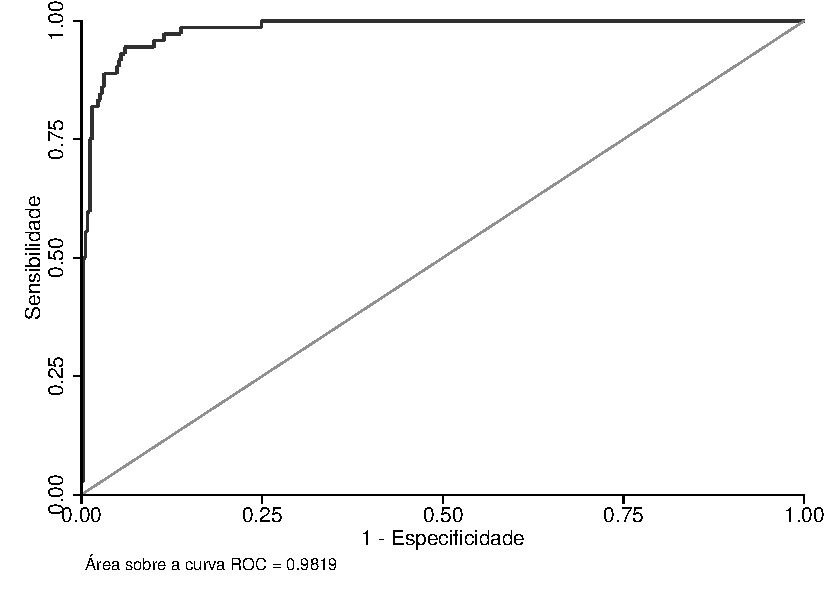
\includegraphics[scale=1]{roc1.pdf}
	\end{center}
	\legend{Fonte: elaboração própria.}
\end{figure}

\end{apendicesenv}
\newpage

% REFERENCIAS
\bibliography{biblio}

\end{document}